\documentclass{iu9lab}

\graphicspath{ {../pics/} }

\worktype{Лабораторная работа}
\title{Базовые средства разработки для языка Java}
\author{Старовойтов А. И.}
\teacher{Посевин Д. П.}
\group{ИУ9-21Б}
\course{Языки и методы программирования}
\labnumber{1}

\begin{document}

\maketitle

\section{Цели}

формирование комфортного окружения для разработки ПО на языке Java.

\section{Задачи}

\begin{itemize}
  \item
        Установка jdk на ваш компьютер
  \item
        Проверка работоспособности jdk
  \item
        Установка IntelliJ IDEA на ваш компьютер
\end{itemize}

\section{Решение}

\subsection{Код}

\begin{lstlisting}[language=java]
import java.util.stream.IntStream ;

public class Factorial {
    public static void main (String[] args) {
        if (args.length == 0) {
            System.out.println("usage: java Factorial x");
        } else {
            int n = Integer.parseInt(args[0]);
            int f = IntStream.range(1, n + 1).reduce(1, (r, x)->r*x);
            System.out.println(f);
        }
    }
}
\end{lstlisting}

\subsection{Скриншоты}

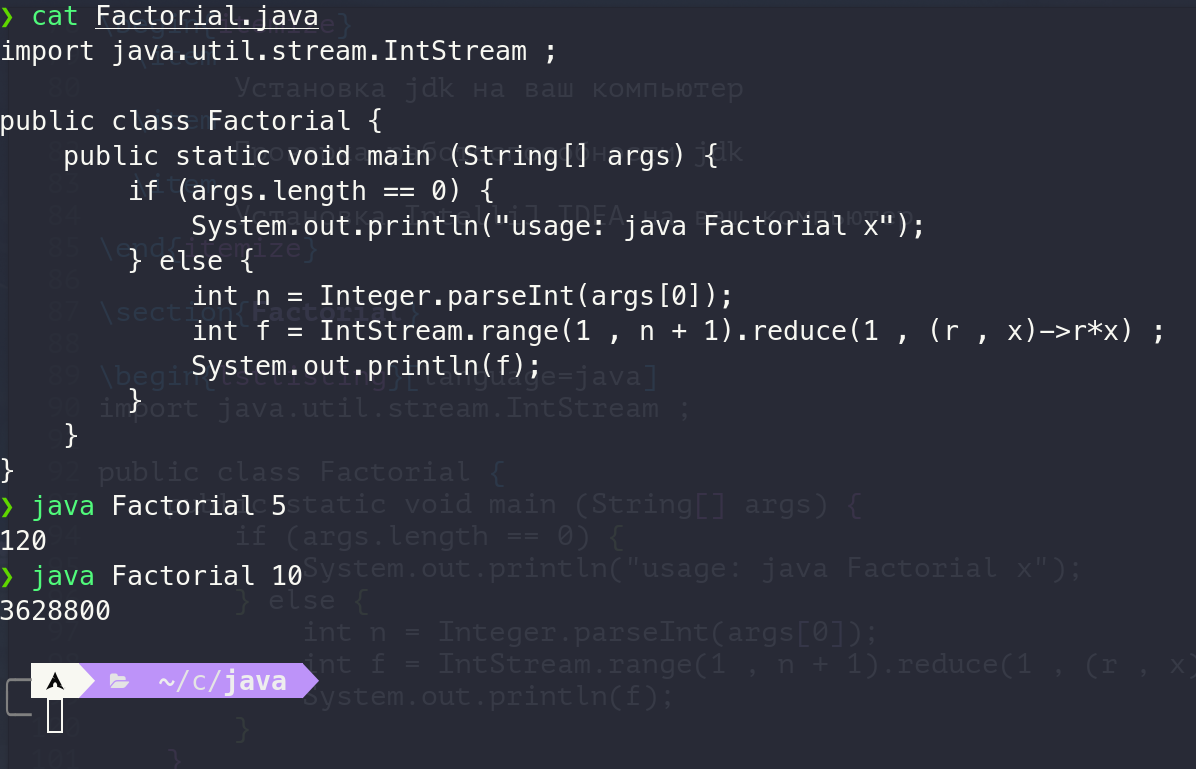
\includegraphics{terminal}
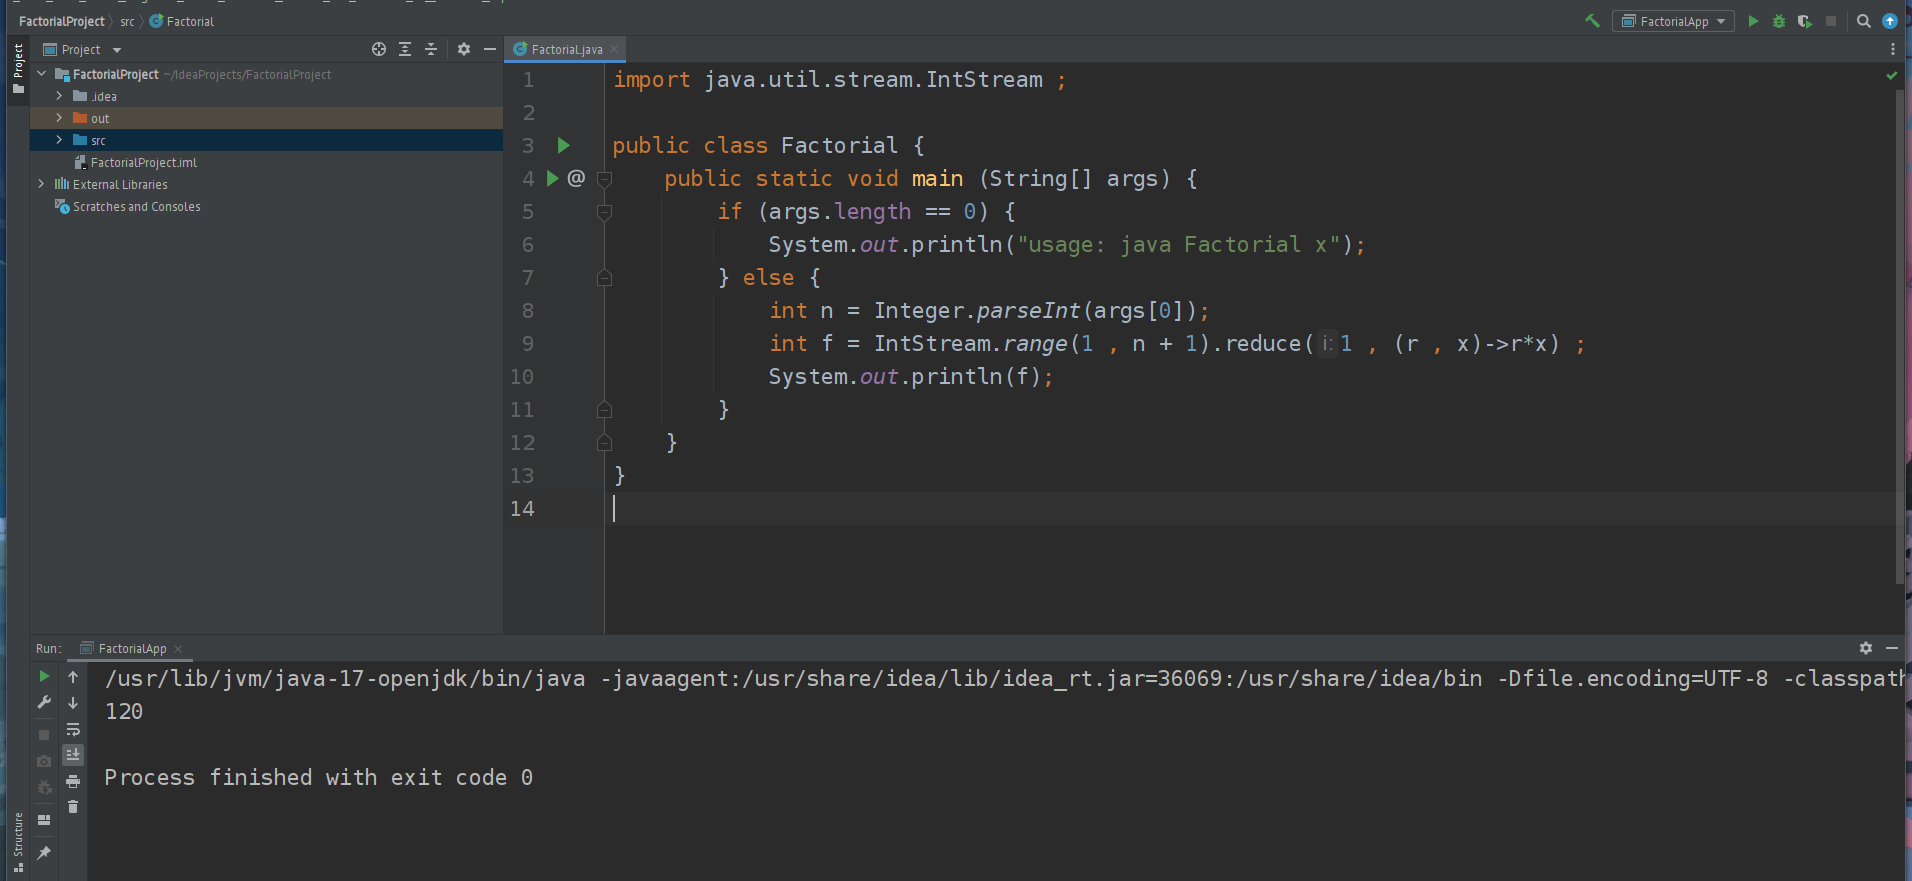
\includegraphics{intellij}
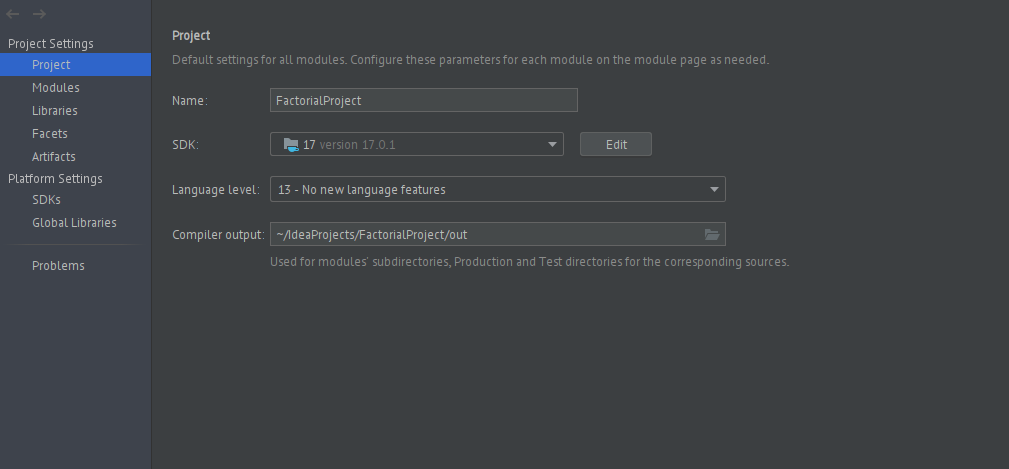
\includegraphics{settings}

\end{document}
